% !TeX root = ../main.tex

\chapter{Verwandte Arbeiten}\label{chapter:background}
	
	%In this chapter, \dots

	%\section{Math} \label{sec:full_grids}
	
		%Math:
		%\begin{align}
			%\Phi(x) = \max(1 - \abs{x}, 0)
		%\end{align}
		
	 %\subsection{Example Figure} \label{sec:back_nodal_hierarchical_basis}
		
		%\begin{figure}[htbp]
			%\centering
			%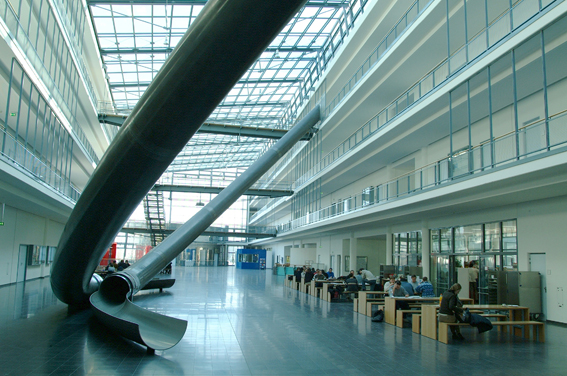
\includegraphics[width=0.5\textwidth]{figures/tum.jpg}
			%\caption{Example picture that was taken from an external source \takenFrom{asc_notes}.}
			%\label{fig:nodalBasis}
		%\end{figure}
		
		%References on figures work like this: blblablabla (see \refFigure{fig:nodalBasis}). If you used external knowledge for a paragraph, use the cite command at the very end of a sentence but right before the full stop \cite{ba_molzer}.
		
		%If you use an $l$ for math symbols, use $\ell$ instead for better readability.
		
	Vor dem Behandeln eines Problems ist es wichtig sich ebenso darüber zu informieren, was in diesem Bereich bereits in anderen Arbeiten behandelt wurde und welche Ergebnisse dabei erzielt wurden. Diese 
	Die Forschungen im Bereich der Platzierung und des Designs von Benutzeroberflächen in Desktop-Anwendungen \todo{Formulieren} Jahrelange Erfahrung
	
	
	Auch mit der Platzierung in virtuellen 3D-Umgebungen haben sich einige Leute beschäftigt. \todo{Beispiele und schöner}
	Zu dem Thema plattformübergreifender Programme in der erweiterten Realität gibt es ebenso schon einige Ansätze \todo{Links}, aber bei näherer Betrachtung dieser Programme fällt auf, dass hierbei häufig auf graphische Benutzeroberflächen weitestgehend verzichtet wurde. 
	- eventuell Verknüpfung zu diegetic?
		
	\section{Priorisieren von Benutzeroberflächen}
		\todo{Abschnitt überprüfen und Beweise einfügen}
		Das Umstrukturieren von Menüs ist nicht trivial, denn jede Veränderung in der Benutzeroberfläche kann das Nutzererlebnis drastisch verändern, falls der Nutzer dadurch irritiert wird. Dies ist sowohl in zweidimensionalen Programmen der Fall, wie auch in der virtuellen dreidimensionalen Welt.\todo{Zitat Aus UX bereich}
		Mit diesem Nutzererlebnis setzt sich seit einigen Jahren der Bereich des UX Designs\todo{UX erklären} auseinander. 
		Ein wichtiger Aspekt davon ist es, dem Nutzer sowohl nicht zu viel als auch nicht zu wenig Informationen auf einmal zu geben. Dies könnte sonst zu einer Überfordert führen, beziehungsweise durch mangelnde Daten die Nutzung erschweren.
		Es gibt für dieses Problem jedoch keine klare Lösung, da es sich dabei um ein subjektives Erlebnis handelt\todo{Link zu UX 1}.
		Um aber das Risiko einer Verschlechterung des Nutzungserlebnisses gering zu halten, hilft es die vorhandenen Informationen zu priorisieren und abhängig davon zu entscheiden, wann und wie diese dem Nutzer angezeigt werden. Dazu verwendet man normalerweise Untermenüs oder Tabs. Alternativ dazu können auch (begriff aus Sonjas quellen) verwendet werden.
		
		- Elemente immer angezeigt (typisch Speichern und Exit)
		- Elemente können versteckt werden (Funktionen Einfügen/Ausschneiden)
		- Elemente in Untermenü (dropdown)
		- elemente in Unteruntermenüs (Funktionen, die selten verwendet werden z.B Einstellungen)
		
		%- UX
		%- Prioritätsgruppen
		%- Umsetzung in 2D
		
	\section{Positionierung in 2D}
		Das verbreitetste Konzept bei der Erstellung von Nutzeroberflächen ist das WIMP-Konzept. Die Abkürzung steht für \term{Windows}, \term{Icons}, \term{Menus} und \term{Pointers}. 
		Damit deutet sie bereits darauf hin, wie man sich die Umsetzung dieses Konzepts vorstellen kann. Programme werden bei dieser nämlich als Fenster dargestellt. Diese können weitere Fenster enthalten oder auch Menüs, in welchen Inhalte angeordnet sind. Um Funktionen möglichst kompakt anzeigen zu können, werden diese teilweise in Form von einem Bild oder Zeichen, einem sogenannten \term{Icon} dargestellt.
		Als Anker zum Positionieren des Fensterinhalts dienen jeweils die Eckpunkte des Fensters. Die einzelnen Elemente werden in den Fenstern also immer relativ zu mindestens einer Ecke des jeweiligen Fensters platziert. Dadurch kann der Inhalt eines Programmfensters bei dessen Verschiebung oder Skalierung mitbeweget werden. Damit ein Objekt sich zudem mit dem enthaltenden Bildausschnitt vergrößert, verkleinert oder darin zentriert bleibt, muss es hingegen an zwei oder mehr Ecken gebunden werden.
		\todo{Bild aus Unity}
		%Damit sich Programmfenster beliebig vergrößern lassen, auch unabhängig von den ursprünglichen Seitenlängenverhältnissen, ohne dass der Inhalt an einer Seite abrupt abgeschnitten wird, muss 
		\todo{Fertigstellen}
		%- Windows Icons Menus Pointers
		
		%- Menüs / Fenster
		%Menüs geben eine Auswahl von Funktionen in Form von ...
		%- Bildschirmränder
		
		
	\section{Positionierung in 3D (VR/AR auch ohne)}
		
		In Programmen, die eine dreidimensionale virtuelle Welt anzeigen (im Folgenden \term{3D-Programm} genannt), wird eine spezielle Form der graphischen Benutzeroberfläche verwendet. Diese liegt nicht in einer zweidimensionalen Ebene vor der Kamera, sondern befindet sich im dreidimensionalen Raum. Dies ermöglicht auch nicht-planare Formen, was dieser Abwandlung den Namen \term{3D User Interface} gab.
		%- 3D Programm: UI in Welt platziert
		- Üblich Hände und Kopf oder an statischen Objekten
		- Beispiele! Zylinderbild
		
		\begin{figure}[htbp]
			\centering
			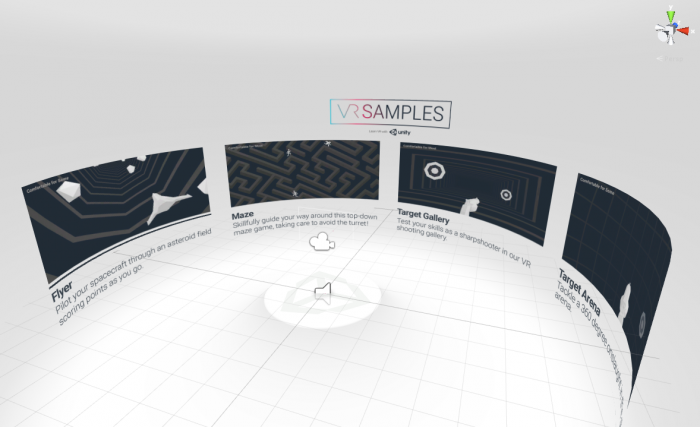
\includegraphics[width=0.75\textwidth]{figures/cylinder_mapping.png}
			\caption{Example picture that was taken from an external source \takenFrom{unityCurved}.}
			\label{fig:cylinder_mapping}
		\end{figure}
		- dreidimensionale Benutzeroberflächen